%%%%%%%%%%%%%%%%%%%%%%%%%%%%%%%%%%%%%%%%%%%%%%%%%%%%%%%%%%%%%%%%%%%%%%%%%%%%%%%%%%%%%%%%%
% Section 4: Xilinx Devices
%	This section contains a description of the following:
%	- Vivado FPGA devices (with terminology)
%	- Device data structures in RapidSmith, 
%	- Device files and XDLRC files  
%	- Step-by-step guide on how to intall new devices  
%%%%%%%%%%%%%%%%%%%%%%%%%%%%%%%%%%%%%%%%%%%%%%%%%%%%%%%%%%%%%%%%%%%%%%%%%%%%%%%%%%%%%%%%%
\newpage
\section{Devices}

\subsection{Xilinx FPGA Architecture Overview} \label{fpgaArch}
This section is intended to give a brief introduction to Xilinx FPGA
architecture and terminology. The terminology introduced here is consistent
with the terminolgy used in the Vivado Design Suite. If you are already familiar
with Xilinx FPGA devices, then you can skip to \autoref{devicesRS2}. 
As you read through this section, it may be helpful to open a sample device in Vivado's
Device Browser. To do this, open a new command prompt and run Vivado in Tcl mode
(``vivado -mode tcl''). Then, run the following commands in the Vivado prompt:

\begin{verbatim}
Vivado% link_design -part xc7a100tcsg324-3 -quiet
Vivado% start_gui
\end{verbatim}

\noindent
After these commands are run, a GUI view should pop up showing the components
of an Artix7 FPGA part. Use this to explore the Xilinx device architecture if
needed.

\subsubsection{Tiles}
Conceptually, a Xilinx FPGA can be thought of as a two dimensional
array of \cls{Tile}s. A \cls{Tile} is a template section within a FPGA that
performs a specific function (say, implementing logic equations). Templates are
then duplicated across the device (all copies are identical) and different
\cls{Tile} types are wired together. As an example, \autoref{fig:tileExample}
displays three types of template \cls{Tile}s in an Artix7 part.

\begin{figure}[H]
 \centering
 \includegraphics[width=0.7\columnwidth]{tiles}
 \caption{Highlighted example \cls{Tile}s in an Artix7 FPGA.}
 \label{fig:tileExample}
\end{figure}

\noindent
The two \pgm{VBRK} \cls{Tile}s on the left are used for intermediate wiring.
The two \pgm{INT\_L} \cls{Tile}s on the right are switchbox \cls{Tile}s.
These are reconfigurable routing \cls{Tile}s that allow a single wire to go
multiple different locations within the FPGA. The two \pgm{CLBLL} \cls{Tile}s
in the middle are used to implement combinational and sequential digital logic.
They are the basic building blocks of Xilinx FPGAs. Other \cls{Tile} types
include DSP, BRAM, and IOB.
 
\subsubsection{Primitive Sites}

\begin{figure}[b!]
\centering
   \begin{subfigure}[b!]{0.65\textwidth}
   \includegraphics[width=1\linewidth]{site}
   \caption{}
   \label{fig:site1} 
\end{subfigure}

\begin{subfigure}[b!]{0.65\textwidth}
   \includegraphics[width=1\linewidth]{subsite}
   \caption{}
   \label{fig:site2}
\end{subfigure}

\caption{(a) A highlighted example of a SLICEL \cls{Site} in a CLBLL \cls{Tile}
of an Artix7 FPGA. (b) The basic components of a \cls{Site} in a
Xilinx FPGA.}
\label{fig:site}
\end{figure}

Each \cls{Tile} can contain one or more \cls{Primitive Site}s (often shortened
to \cls{Site}). As \autoref{fig:tileExample} shows, CLBLL \cls{Tile}s
have two \cls{Site}s, INT\_L \cls{Tile}s have one \cls{Site}, and VBRK \cls{Tile}s
have none. A \cls{Site} is the part within a \cls{Tile} that actually performs
its ``useful'' function. The remainder of the \cls{Tile} is used to wire signals
to/from its \cls{Site}s. \autoref{fig:site} shows a SLICEL, one of the
\cls{Site}s within a CLBLL \cls{Tile}. As the figure shows, there are three main
components to \cls{Site}s in Xilinx FPGAs:

\begin{itemize}
  \item \cls{Site} \cls{PIP}s: Reconfigurable routing PIPS used for intrasite
  routing (also called routing muxes). In Vivado, \cls{Site} \cls{PIP}s are usually configured
  automatically as cells in a design are being placed (based on cell properties
  and placement location).
  \item \cls{BEL}s: \pgm{B}asic \pgm{EL}ements are hardware components within
  the \cls{Site} for implementing digital logic. For example, LUT \cls{BEL}s within a SLICEL
  are used to implement logic equations, and Flip Flop \cls{BEL}s are used
  as storage. In a synthesized netlist, design elements are mapped to physical
  \cls{BEL}s during implementation.
  \item \cls{Site Pin}s: \cls{Site} input and output. These pins are connected
  to \cls{Wire}s of the parent \cls{Tile} and typically drive general
  fabric.
\end{itemize}

\subsubsection{Wires and PIPs} \label{wireSection}
 
FPGA components are connected together using metal \cls{Wire}s (called
\cls{Node}s in Vivado). In order to make the FPGA reconfigurable,
\cls{Wire}s are connected together through Programmable Interconnect Points
(\cls{PIP}s). Individual \cls{PIP}s can be enabled or disabled as a design is
being routed, and a string of enabled \cls{PIP}s uniquely identify the
used \cls{Wire}s of a physical route. \cls{PIP}s are most commonly
found in Switchbox \cls{Tile}s, and enable a single wire to be routed to many
different locations in the FPGA. \autoref{fig:switchboxPIP} shows an
example of a switchbox.

\begin{figure}[H]
	\centering
	\includegraphics[width=0.45\columnwidth]{pipExample}
	\caption{An example of PIP wire connections in a device. The green wire
	represents the source wire, and the red wires represent all possible sink
	wires in the Switchbox. The highlighed white sections of the figure are PIP
	connections.}
	\label{fig:switchboxPIP}
\end{figure} 
 
\subsection{Device Data Structures} \label{devicesRS2}
In the original RapidSmith, the \cls{Device} architecture stopped at the
\cls{Site} level. A \cls{Site} was considered a black box who could be
configured using string attributes, but the actual components were unknown.
RapidSmith 2 extends the \cls{Device} architecture to include all components
\pgm{within} a \cls{Site} as well. \autoref{fig:deviceDataStructures}
shows the new data structure hierarchy, which can be found in the {\em
edu.byu.ece.rapidSmith.device} package.

\begin{figure}[H]
	\centering
	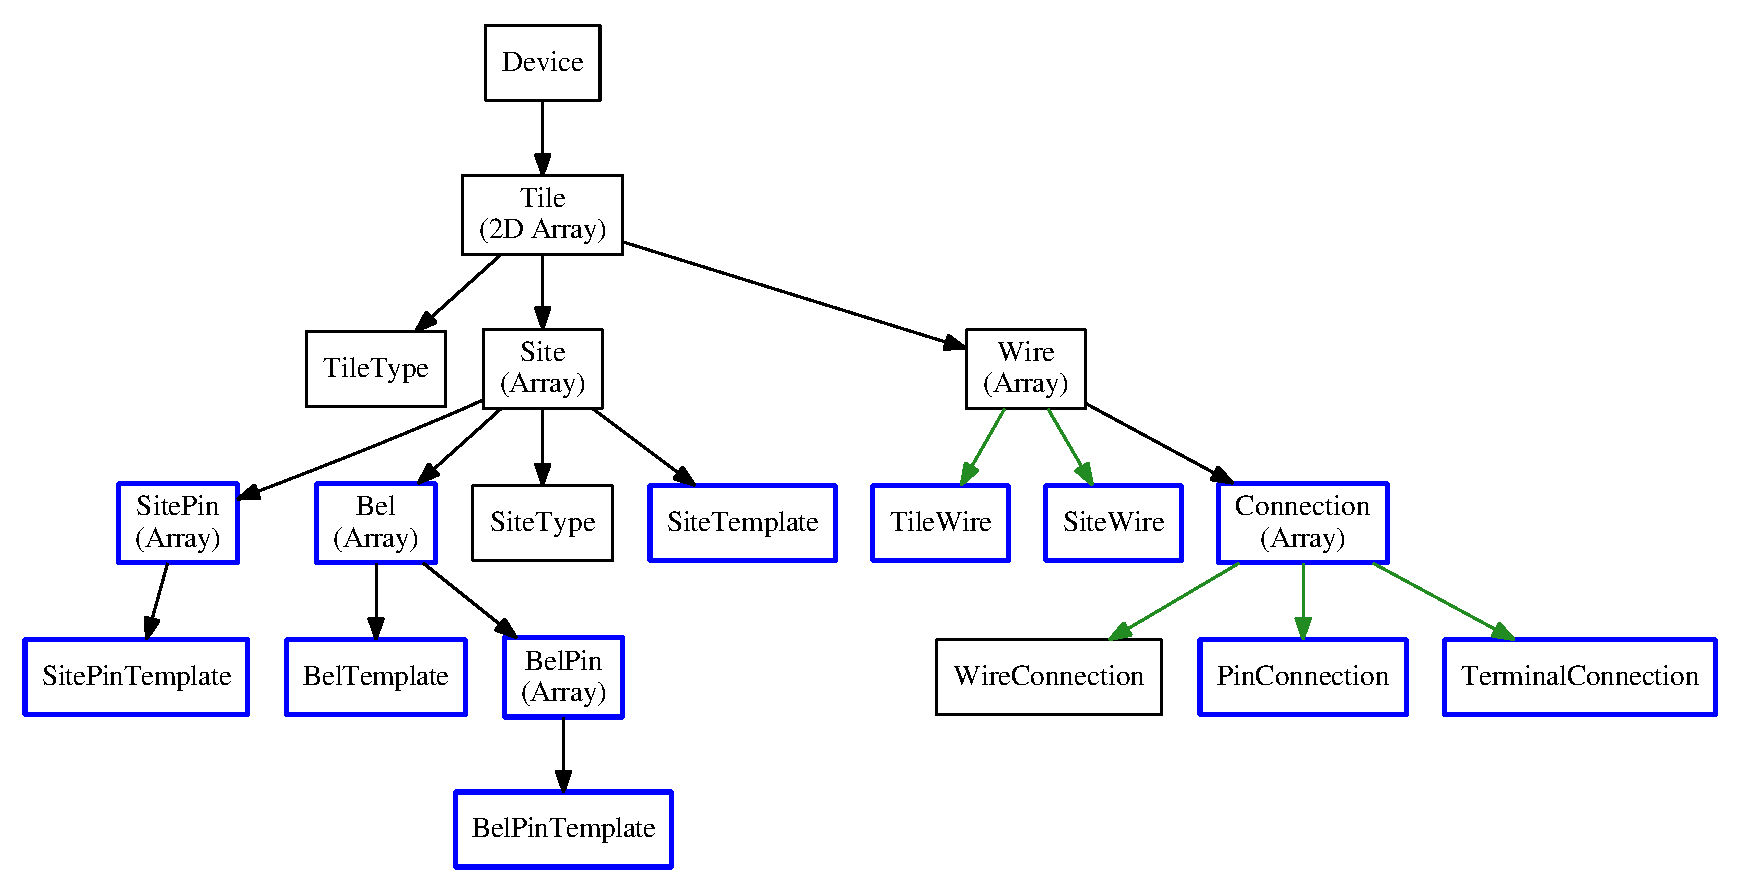
\includegraphics[width=1\columnwidth]{deviceDS.eps}
	\caption{RapidSmith2 \cls{Device} data structure tree. Green arrows represent
	inheritance, and black arrows represent association. Classes and Interfaces
	bolded in blue are new to RapidSmith 2.}
	\label{fig:deviceDataStructures}
\end{figure}

\noindent
The classes and interfaces within {\em edu.byu.ece.rapidSmith.device} are named
to reflect the terminology used by Xilinx. Many classes that exist in Vivado's
Tcl interface have a direct map to a class in RapidSmith (such as a \cls{Tile}).
Because of this, most RapidSmith data structures represent a straightforward
part of a Xilinx FPGA, The reader is referred to the documentation in the
source code to learn more about each data structure. Also, The
\pgm{DeviceBrowser} and \pgm{DeviceAnalyzer} programs described in 
\autoref{examples} illustrate how to load and browse a device down to the
\cls{Tile} and \cls{Site} levels.

\subsubsection{Templates}
As \autoref{fig:deviceDataStructures} shows, there are several template
classes in RapidSmith. Template classes are used to specify the configuration of
certain structures only once, and then reuse the configuration across
identical objects. The usefulness of templates is best shown with an example. In
an Artix-7 {\em xc7a100tcsg324} part, there are 11,100 \cls{Site}s of type
SLICEL. Each of these SLICELs have 215 \cls{BEL}s, \cls{Site} \cls{Pin}s, and
\cls{Site} \cls{PIP}s combined. In order to save memory, RapidSmith
lazily creates these objects only when a SLICEL \cls{Site} is being used. The
alternative would be to create each of the objects when a device is loaded.
Template classes should \pgm{NOT} be used by the normal user. When creating
algorithms using RapidSmith's API, use the non-template version of classes.

\subsubsection{WireEnumerator} \label{wireEnum}
Wires with the same name can occur several times throughout a Xilinx FPGA
device. For example, the wire ``CLBLL\-\_L\_C2'' exists in every \cls{Tile} of
type ``CLBLL\_L''. In order to make the device files small, each uniquely named \cls{Wire}
is assigned an integer enumeration. This avoids moving strings around in
memory which would be costly in terms of both space and comparison times.
RapidSmith manages all uniquely named wires in an FPGA family with a
\cls{WireEnumerator}. The \cls{WireEnumerator} class has methods that convert to
and from the wire name and enumeration of a \cls{Wire}, and also stores other
\cls{Wire} information such as direction and type. In previous versions of
RapidSmith, the user had to use the \cls{WireEnumerator} extensively while
building CAD tools. RapidSmith 2 has changed this, largely abstracting the
\cls{WireEnumerator} away in favor of more convenient methods in all classes and
interfaces that deal with \cls{Wire}s. For example, the name or enumeration of a
\cls{Wire} can now be obtained with the function calls {\em Wire.getWireName()}
and {\em Wire.getWireEnum()} respectively. A handle to the
\cls{WireEnumerator} still exists in the \cls{Device} class for those who
want to use it, but this is not recommended. 

\subsubsection{TileWire and SiteWire} \label{wires}
\cls{Wire}s in RapidSmith are uniquely identified not only by their name
(or enumeration), but also by the \cls{Tile} or \cls{Site} in which they exist.
RapidSmith 2 introduces the \cls{TileWire} and \cls{SiteWire} classes to
encapsulate this information for the user. Many functions in RapidSmith now
return a \cls{TileWire} or \cls{SiteWire} (wrapped in a generic \cls{Wire}
object) to the user instead of an integer wire enumeration.

\subsubsection{Wire and Connection Interfaces}
As \autoref{fig:deviceDataStructures} shows, there are two classes that
inherit the \cls{Wire} interface (described in \autoref{wires}) and
three classes that inherit the \cls{Connection} interface (described in 
\autoref{otherConns}). In general, most methods in RapidSmith return the
generic interface instead of the subclasses. When creating CAD tools in
RapidSmith, it is suggested that the user use these interfaces. Several of the
examples referenced in \autoref{examples} demonstrate the use of these
interfaces.

\subsection{Device Files}
The \cls{Device} data structures in RapidSmith are created from XDLRC files.
For older Xilinx parts (series 7 and below), these files can be created
in ISE with the {\em xdl} command. For newer parts (ultrascale and
above), XDLRC files can be created in Vivado using the TINCR command
{\em tincr\-::write\_xdlrc}. Because XDLRC files can
grow to be hundreds of Gigabytes in size, RapidSmith compresses them into much
smaller device files (usually in the tens of Megabytes) and stores those
instead. This section gives a brief overview of the syntax of XDLRC files, and
how to install new device files in RapidSmith from both ISE and Vivado.

\subsubsection{Basic Syntax of XDLRC files}
In general, users of RapidSmith do not need to understand the syntax of XDLRC
files to create CAD tools in RapidSmith. The syntax is introduced here for those
who are interested, and for those who want to modify the XDLRC parser
in some way. If these don't apply to you, then go ahead and skip this section.
XDLRC files are textual descriptions of Xilinx FPGA devices and can be very
verbose (which is why they get so large). This section highlights the main parts
of an XDLRC file with accompanying images. As you will see, much of the
terminology is the same as \autoref{fpgaArch}.

\bigbreak \noindent
\begin{large}
\pgm{Tiles}
\end{large}

\begin{figure}[H]
	\centering
	\includegraphics[width=1\columnwidth]{xdlrcTile}
	\caption{Tile syntax in XDLRC files}
	\label{fig:xdlrcTile}
\end{figure}

\noindent
A tile in an XDLRC file corresponds to the same thing as the \cls{Tile}
described in \autoref{fpgaArch}. Each tile is declared with a ``(tile''
directive as shown above followed by the unique row and column index of where
the tile fits into the grid of tiles found on the FPGA. The tile declaration
also contains a name followed by a type with the final number being the number
of primitive sites found within the tile. The tile ends with a ``tile\_summary''
statement repeating the name and type with some other numbered statistics.
Tiles can contain three different sub components, primitive sites, wires, and
PIPs.

\bigbreak \noindent
\begin{large}
\pgm{Primitive Sites}
\end{large}

\begin{figure}[H]
	\centering
	\includegraphics[width=1\columnwidth]{xdlrcSite}
	\caption{Primitive site syntax in XDLRC files}
	\label{fig:xdlrcSite}
\end{figure}

\noindent
Primitive site declarations in XDLRC files contain a list of pinwires which
describe the name and direction of pins on the primitive site. The first
pinwire declared in the example above is the BX input pin which is the internal
name to the SLICEL primitive site. Pinwires have an external name as well to
differentiate the multiple primitive sites that may be present in the same
tile. In this case, BX of SLICE\_X9Y127 has the external name BX\_PINWIRE3. In
RapidSmith, only the first pin name (i.e. BX above) is used.

\bigbreak \noindent
\begin{large}
\pgm{Wire}
\end{large}

\begin{figure}[H]
	\centering
	\includegraphics[width=1\columnwidth]{xdlrcWire}
	\caption{Wire syntax in XDLRC files}
	\label{fig:xdlrcWire}
\end{figure}

\noindent
A wire as declared in XDLRC is a routing resource that exists in the tile that
may have zero or more connections leaving the tile. In the example above, the
wire ``E2BEG0'' connects to 5 neighboring tiles. These connections (denoted
by ``conn'') are described using the unique tile name and wire name of that tile
to denote connectivity. The connections are not programmable, but hard wired
into the FPGA. Wire portions of the XDLRC file are included in the definition of
every tile (even if the same tile type has already been printed), which has a
big impact on the final size of XDLRC files. How RapidSmith handles wire
duplication is described in \autoref{wireEnum}. The \cls{WireConnection}
objects that are created from this part of the XDLRC are described in
\autoref{wireConnSection}.

\bigbreak \noindent
\begin{large}
\pgm{PIP}
\end{large}

\begin{figure}[H]
	\centering
	\includegraphics[width=1\columnwidth]{xdlrcPip}
	\caption{PIP syntax in XDLRC files}
	\label{fig:xdlrcPip}
\end{figure}

\noindent
A PIP (programmable interconnect point) is a possible connection that can be
made between two wires. In the example above, the PIP is declared in the tile
and repeats the tile name for reference. It specifies two wires by name that
both exist in that same tile (``BEST\_LOGIC\_OUTS0'' and ``BYP\_INT\_B5'') and
declares that the wire ``BEST\_LOGIC\_OUTS0'' can drive the wire
``BYP\-\_INT\_B5''. A collection of these PIPs in a net define how a net is
routed and is consistent with saying that those PIPs are �turned on.�
\autoref{wireConnSection} describes in detail how PIPs are represented in
RapidSmith.

\bigbreak \noindent
\begin{large}
\pgm{Primitive Definitions}
\end{large}

\bigbreak \noindent
The Primitive Definition portion of an XDLRC file textually describes the
components found within a \cls{Primitive} \cls{Site} (a SLICEL for example)
and how they are connected. \cls{BEL}s, \cls{Site} \cls{Pins}, \cls{Site}
\cls{PIP}s, configuration options, and route-throughs are the elements that are
most commonly found within a primitive definition. An example of a complete
primitive definition file of type BUFHCE can be seen in
\autoref{fig:xdlrcDef}. The sub-site data structures in RapidSmith (\cls{Bels},
\cls{SiteWire}s, etc.) are built by parsing this section of the XDLRC file.

\begin{figure}[H]
	\centering
	\includegraphics[width=1\columnwidth]{xdlrcDef}
	\caption{Primitive Def sections of XDLRC files}
	\label{fig:xdlrcDef}
\end{figure}